\documentclass{beamer}
\usepackage{HECbeamer}
% \usepackage{pgfpages}
% \pgfpagesuselayout{4 on 1}[letterpaper, landscape, border shrink=5mm]
\title[\color{white}{MATH60619A \S~7 - Introduction to mixed effects models}]{\texorpdfstring{MATH60619A \\Statistical analysis and inference \\ \S~7 - Introduction to mixed effects models}{MATH60619A \\Statistical analysis and inference \\ \S~7 - Introduction to mixed effects models}}
\author{Léo Belzile}
\institute{HEC Montréal\\
Department of Decision Sciences}
\date{} 

\begin{document}
\frame{\titlepage}

% \begin{frame}
% \frametitle{Overview of course material}
% \begin{center}
% \includegraphics[scale=0.35]{Figures/fig6.png}
% \end{center}
% \end{frame}


\begin{frame}[fragile]
\frametitle{Chapter overview}


\begin{tcolorbox}[colback=white, colframe=hecblue, title=Chapter 7 - Introduction to mixed effects models]
% 
\vp \vp
\tableofcontents
\end{tcolorbox}
\end{frame}
\section{Inclusion of group effect for the mean}
\begin{frame}
 \frametitle{Inclusion of group effects}
 \bi 
 \item So far, we have only accounted for group structure by modelling the within-group correlation.
 \item We may also want to include a \alert{group effect} in the mean model, i.e., a different intercept for each group.
 \item This is done by adding the categorical group variable \texttt{g} as explanatory variable in the mean model, which translates into $m-1$ indicator variables $\I{\code{g}=i}$ for $i=1, \ldots, m-1$ if there are $m$ groups. 
 \item Suppose that we only include the categorical variable \code{g} representing groups,
 \[ Y_{ij}= \beta_0 + \sum_{i=1}^{m-1} \beta_i\I{\code{g}=i} + \eps_{ij},\]
 \bi \item for the baseline (group $m$), the intercept is $\beta_0$,
 \item the group effect for $\code{g}=i$ is $\beta_i$ $(i=1, \ldots, m-1)$, and the overall group-specific ``intercept'' is $\beta_0+ \beta_i$.
 \ei
 \ei
 
 \end{frame}
 
\begin{frame}
\frametitle{Linear model with a group effect for the \texttt{revenge} data}
We consider a regression model for \texttt{revenge} with a group effect to illustrate the challenges.
\bi
\item The idea here is to model the fact that desire for revenge can vary between subjects.
\item In the current example, there are only five observations per person to estimate the group effect.
% \item To do this, we can use a model that includes a different parameter for each person. 
\item The model will ignore the within-person correlation for now.
% \item First we'll see how to fit a model with a group (or subject) effect without correlation.
% \item We will include the correlation in this model later on.
\ei
\end{frame}




\begin{frame}[fragile]
\frametitle{Model with fixed effects for subject}
\begin{tcolorbox}[colback=white, colframe=hecblue, title=\SASlang{} code to fit a linear model via REML]
\begin{verbatim}
proc mixed data=revenge method=reml; 
class id; 
model revenge = id sex age vc wom t / solution; 
run;
\end{verbatim}
\end{tcolorbox}
{\footnotesize In addition to the categorical variable \code{id}, the model includes the same explanatory variables as before. Each person has his/her own ``intercept'' parameter (\texttt{id=80} is the baseline category). 


}
\end{frame}

 \begin{frame}
\frametitle{Estimates of fixed effects}
\begin{center}
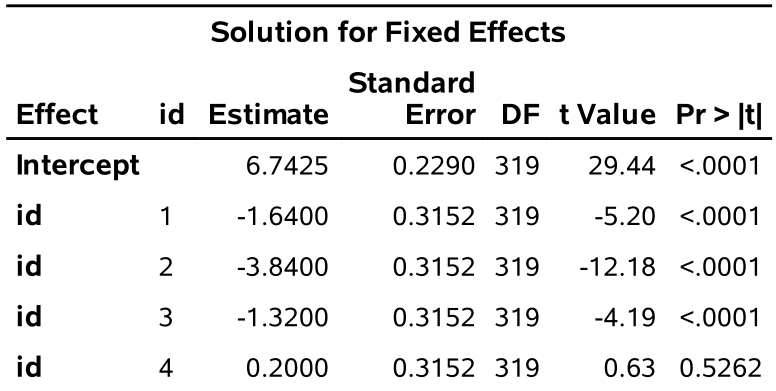
\includegraphics[width = 0.6\linewidth]{img/c6/slides7-e01}
\begin{align*}
\vdots      \end{align*}



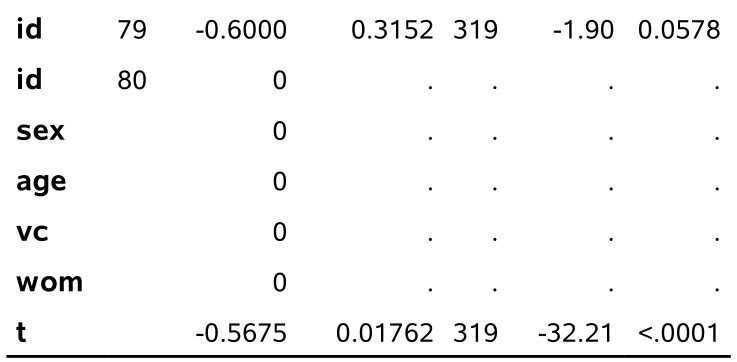
\includegraphics[width = 0.6\linewidth]{img/c6/slides7-e02}
\end{center}

\end{frame}

%  \begin{frame}
% \frametitle{\SASlang{} output}
% \textbf{Estimates of fixed effects (continued)}
% \begin{center}
% \includegraphics[scale=0.35]{Figures/long53.pdf}
% \end{center}
% \end{frame}

 \begin{frame}
\frametitle{Parameter significance}
\begin{center}
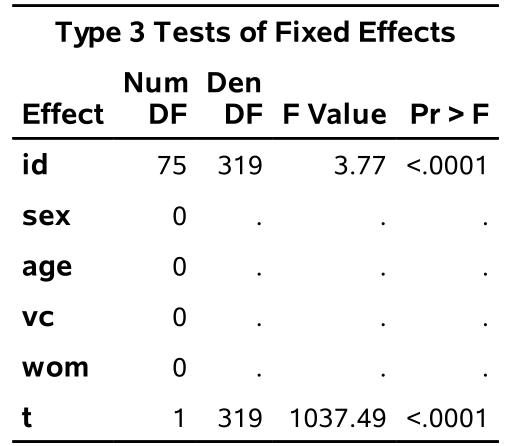
\includegraphics[width=0.4\linewidth]{img/c6/slides7-e03}
\end{center}
{\footnotesize 


There are \textbf{no} parameters estimates or tests for the variables \code{sex}, \code{age}, \code{vc} or \code{wom}, but there is for the time variable \code{t}. 
Because some covariates are fixed over time, their effect are not uniquely estimable (perfect collinearity). If we remove \code{id} from the model, we can however estimate their effects (hence $75$ \code{df} rather than $79$ in the $F$-table).

}
\end{frame}


\begin{frame}[fragile]
\frametitle{Collinearity}
\bi
\item  Once we've included a fixed effect for each person, \alert{it is impossible to include any variable that does not vary in time for a single person}. 
\item The variables \code{sex}, \code{age}, \code{vc} and \code{wom} are fixed in time for each person (\code{vc} and \code{wom} were only measured once, at time 1). 
\item These variables are already implicitly included in the individual effect. There is \alert{perfect collinearity} between a variable fixed in time, and the \code{id} variable. 
\item This means that we can perfectly predict the value of \code{sex} (and the three others) by only looking at the \code{id} variable. 
\item Therefore, we cannot have a fixed effect for each individual while simultaneously including variables that are fixed in time for each subject.
\ei
\end{frame}
 \begin{frame}
 \frametitle{Challenges arising from the inclusion of a group effect}
 
 \bi 
 \item Group is a categorical variable: we need enough observations in each group to reliably estimate the group effects.
 \item If the number of groups $m$ is large relative to the overall sample size, there may also be too many parameters in the model. 
 \item We cannot estimate the effect of variables that do not vary within group if we add group effects.
  \ei
\end{frame}


%  \begin{frame}
% \frametitle{\SASlang{} output}
% \textbf{Estimates of fixed effects (continued)}
% \begin{center}
% \includegraphics[scale=0.45]{Figures/long55.pdf}
% \end{center}
% \bi
% \item Each person has his/her own parameter (except for id=80, the reference category). 
% \item There are \alert{no} parameters or tests for the variables \code{sex}, \code{age}, \code{vc} or \code{wom}. But there is for the time variable \code{t}. 
% \item \textbf{\alert{What happened? }}
% \ei
% 
% \end{frame}

% 
% \begin{frame}[fragile]
% \frametitle{Model with fixed effects for subject}
% \bi
% \item  More generally, with correlated observations within groups, if we add a fixed effect for each group, \alert{we cannot include other variables that do not vary within group}.
% \ei
% \end{frame}

\begin{frame}[fragile]
\frametitle{Model with group effect and correlation structure}
The model fitted next includes only \code{id} and the time variable \texttt{t} as explanatory variables in the mean model, but we specify in addition an $\mathsf{AR}(1)$ correlation structure within-individual for the errors $\bs{\eps}$.

\begin{tcolorbox}[colback=white, colframe=hecblue, title=\SASlang{} code to include a group effect with $\mathsf{AR}(1)$ correlation]
\begin{verbatim}
proc mixed data=revenge method=reml; 
class id tcat; 
model revenge = id t / solution; 
repeated tcat / subject=id type=ar(1); 
run;
\end{verbatim}
\end{tcolorbox}
{\footnotesize  The effect of the $\mathsf{AR}(1)$ correlation parameter is significant (likelihood ratio test statistic of $21.68$, negligible $p$-value under $\chi^2_1$). The estimate of the time effect is $-0.5684$, very close to that we got in the model including \code{sex}, \code{age}, \code{vc} and \code{wom}, and the  $\mathsf{AR}(1)$ structure model in the previous chapter. 

}
\end{frame}
% 
% \begin{frame}
% \frametitle{\SASlang{} output}
% \textbf{Estimates of covariance/correlation parameters}
% \begin{center}
% \includegraphics[scale=0.4]{Figures/long56.pdf}
% \includegraphics[scale=0.4]{Figures/long57.pdf}
% \end{center}
% \bi
% \item 
% \ei
% \end{frame}

% \begin{frame}
% \frametitle{Estimates of fixed effects}
% \begin{center}
% \includegraphics[scale=0.35]{Figures/long58.pdf}
% \end{center}
% \end{frame}
% 
% \begin{frame}
% \frametitle{Estimates of fixed effects (continued)}
% \begin{center}
% \includegraphics[scale=0.32]{Figures/long59.pdf}
% \end{center}
% \end{frame}
% 
% \begin{frame}
% \frametitle{Estimates of fixed effects (continued)}
% \begin{center}
% \includegraphics[scale=0.32]{Figures/long60.pdf}
% \end{center}
% \end{frame}
% 
% \begin{frame}
% \frametitle{Estimates of fixed effects (continued)}
% \begin{center}
% \includegraphics[scale=0.35]{Figures/long61.pdf}
% \end{center}
% \bi
% \item Estimates of parameters for time $23$--$78$ are omitted, but they are non-zero.
% \item The global effect of \code{id} is significant, as well as the effect for time. 
% \item 
% \item In that model, the effect of time was estimated as $-0.5686$.
% \ei
% \end{frame}

\begin{frame}[fragile]
\frametitle{Remark on model comparison}
\bi
\item We have to be careful \alert{not to use} the \ensuremath{\mathsf{AIC}}{} and \ensuremath{\mathsf{BIC}}{} reported in the output to compare this model to the earlier one including \code{sex}, \code{age}, \code{vc} and \code{wom}, since we used the REML estimation method (the default). 
\item \ensuremath{\mathsf{AIC}}{} and \ensuremath{\mathsf{BIC}}{} obtained through REML, are \textbf{not comparable} if the ``mean'' parts of the models (fixed effects) are not the same. 
\item If we want to compare these models, we must use the maximum likelihood estimator (option \texttt{method=ml} when calling \code{proc mixed}). 
\ei
 \begin{center}
  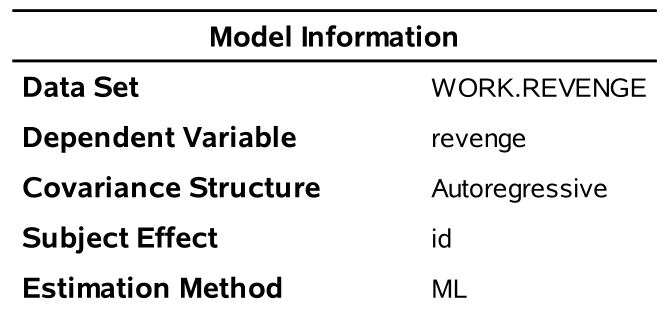
\includegraphics[width = 0.5\linewidth]{img/c6/slides7-e05}
 \end{center}
   
\end{frame}


\begin{frame}[fragile]
\frametitle{Remark on model comparison}
We fit both models with an $\mathsf{AR}(1)$ structure for the errors using maximum likelihood.
\begin{center}
\begin{tabular}{c c c r}
\toprule 
\textbf{Model} & \textbf{AIC} & \textbf{BIC} & $\hat{\rho}$ ($p$-value)\\ \midrule 
\code{sex}, \code{age}, \code{vc}, \code{wom}, \code{t} & 666.1 & \alert{685.1}  & $0.48$ ($10^{-20}$) \\
\code{id}, \code{t} & \alert{653.4} & 851.1 & $-0.013$ ($0.83$)\\ \bottomrule
\end{tabular}
\end{center}
\bi
\item The preferred model according to $\mathsf{AIC}$ includes \code{id}, but $\mathsf{AIC}$ tends to select complicated models.
\item The preferred model according to $\mathsf{BIC}$ includes \code{sex}, \code{age}, \code{vc} and \code{wom} and throws away the \code{id} variable.
\item Once we include an individual effect for group, the correlation
structure seems to be unnecessary --- the estimated coefficient is even negative, which is counter-intuitive and suggests the model is over-parametrized.
\ei
\end{frame}

\begin{frame}
\frametitle{Remark on model comparison}
\bi
\item The choice of covariates depends on the type of study. If we're interested in studying the effects of one or more of the variables \code{sex}, \code{age}, \code{vc} or \code{wom}, then we don't have any choice: we must choose a model that contains all of them. 
\item If we're only interested in the time effect, then the two models will come to the same conclusion either way.
 \item Often, the optimization routine fails --- we cannot estimate both the $\bs{\beta}$ and the covariance matrix parameters.
\item It is possible to include variables that are fixed within group (within person in our example) \textbf{and} group effects (\code{id} in our example) at the same time by using \alert{random effects}.
\ei
\end{frame}
% 
% \begin{frame}
% \frametitle{Chapter overview}
% 
% 
% \begin{tcolorbox}[colback=white, colframe=hecblue, title=Chapter 7 - Models for longitudinal and correlated data]
% \bi
% 
% \begin{tiny}
% \item[1.] Introduction and example
% \item[2.] Covariance and correlation matrix
% \item[3.] Linear model with correlated errors
% \item[4.] Choice of covariance structure
% \item[5.] Hypothesis testing on the covariance structure
% \item[6.]  Linear model with correlated errors and a group effect
% \item[7.] \textbf{\alert{Random intercept model}}
% \item[8.]  Random slope model
% \item[9.] Prediction
% \item[10.] Example of a model with a more complex covariance structure
% \end{tiny}
% \ei
% \end{tcolorbox}
% \end{frame}



% 
% \begin{frame}
% \frametitle{Review: the big picture}
% \bi
% \item We will see, \textbf{step by step}, how to get to a random effects model (optimal model for our problem)
% \item To do this, we will see how to fit the models we just listed
% \item \alert{Option 1}: regression model with correlation structure on the error terms $\varepsilon$
% \item \alert{Option 2}:  regression model with correlation structure on the error terms \alert{\textbf{and}} a group effect
% \item \alert{Option 3}: random effects model
% \bi
% 
% \item We just saw options 1 and 2:
% \ei
% \item \alert{\textbf{We will now see option 3}}
% \ei
% \end{frame}  



\section{Random effect models}
% \begin{frame}[fragile]
% \frametitle{Option 3: Random effects models}
% \bi
% \item  We will see this in detail later, but if we want to include a random effect in the model, this can be done in a few different ways:
% \bi
% 
% \item We can put a random effect on the intercept $\beta_0$
% \item We can put a random effect on $\beta_0$ as well as on the $\beta$ coefficient of certain predictor variables.
% \ei
% \item We will see both kinds of models (the second being an extension of the first) in the next two sections.
% \item We only consider for now models with a random effect on the intercept
% \item \textbf{Terminology}: we will use the terms \alert{random effects model} and \alert{mixed model} interchangeably.
% \bi
% \item The term \alert{mixed model} refers to a model that contains both fixed and random effects. 
% \ei
% \ei
% \end{frame}  
% 
% \begin{frame}
% \frametitle{Random effect models}
% \bi \item The term \textbf{random effect models} (or mixed models) contain individual effects for groups in addition to the usual (fixed effects) of $\mathbf{X}$ --- the $\bs{\beta}$.
% \item Contrary to the previous case, these effects are latent variables (much like residuals) and are not estimated.
%  \item The term \alert{mixed model} refers to a model that contains both fixed and random effects. 
%  
%  \ei 
% \end{frame}
% 


% 
% \begin{frame}[fragile]
% \frametitle{Introduction to random effects models}
% \bi
% \item  We've seen how to do valid statistical inference for the effects of the predictor variables, i.e., the $\beta$ coefficients when the observations are \alert{not independent}. 
% \item We saw that it's possible to estimate the within-group covariance structure and that \SASlang{}  allows a lot of flexibility in terms of covariance structures. 
% \item The choice of covariance structure can be based on criteria like AIC or BIC. We can even test the parameters in the covariance structure between nested models.
% \ei
% \end{frame}

\begin{frame}
\frametitle{Introduction to random effects models}
 Random effects give another way of accounting for within-group correlation and allows prediction of group-level effects in addition to population-level effects.
 \bi \item The main characteristic of the \alert{linear mixed model} is to allow certain variables to have \alert{random effects}, i.e., \alert{to have parameters that vary from one group to another} (from one person to another in repeated measures data). 
\item While each group is allowed an individual effect, the overall average of these effects is zero.
\ei
\end{frame}

% \begin{frame}[fragile]
% \frametitle{Example}
% \bi
% \item  The last example contained longitudinal data, i.e.,  measures taken at multiple time points on the same person. 
% \item The correlation was \alert{within-person} correlation. 
% \item Situations where observations are correlated can appear in other contexts too, including situations where measurements are taken at only one time point. We will see an example where the data are correlated within group.
% \ei
% \end{frame}

\begin{frame}[fragile]
\frametitle{Example: worker motivation}
We consider an example of clustered data.
\bi
\item  A large business collected data about its employees through a questionnaire. 
\item In this example, the response variable is \alert{worker motivation}. 
\item The level of worker motivation is defined as the \textbf{sum} of three items, namely
\bi

\item I share several of the company's values.
\item I feel loyal to the company.
\item I'm proud to tell people what company I work for.
\ei
measured on a Likert scale, ranging from strongly disagree ($1$) to strongly agree ($5$).
\item These data originates from

\begin{quote}
Lee, H.-J. and Peccei, R. (2007). \textsl{Organizational-Level Gender Dissimilarity and
Employee Commitment}. British Journal of Industrial Relations, \textbf{45}, 687--712.
\end{quote}
\ei
\end{frame}

\begin{frame}[fragile]
\frametitle{\texttt{motivation} data}
 The data are found in the file \code{motivation.sas7bdat} and contains the variables%, and the \SASlang{} code in \code{chapter7.sas}. 
\bi

\item \code{nunit}: number of employees in the unit (department).
\item \code{idunit}: id of unit in which the employee worked.
\item  \code{idemployee}: id of employee (within unit).
\item \code{yrserv}: years of service of employee.
\item \code{sex}: sex of employee, either male (\texttt{0}) or female (\texttt{1}).
\item  \code{agemanager}: age of the unit manager (in years).
\item \code{motiv}: worker motivation score.
\ei

\bi
\item  One possible source of correlation between observations is the \alert{unit (or department)} (group variable). 
\item It's possible that motivation is affected by what unit an employee belongs to due to factors such as temperature or type of work, among other things.
\ei
\end{frame}

\begin{frame}[fragile]
\frametitle{Summary statistics}
In the \texttt{motivation} data, units have different number of employees.
For example, unit $1$ has nine employees (three women and six men). 
\begin{center}
 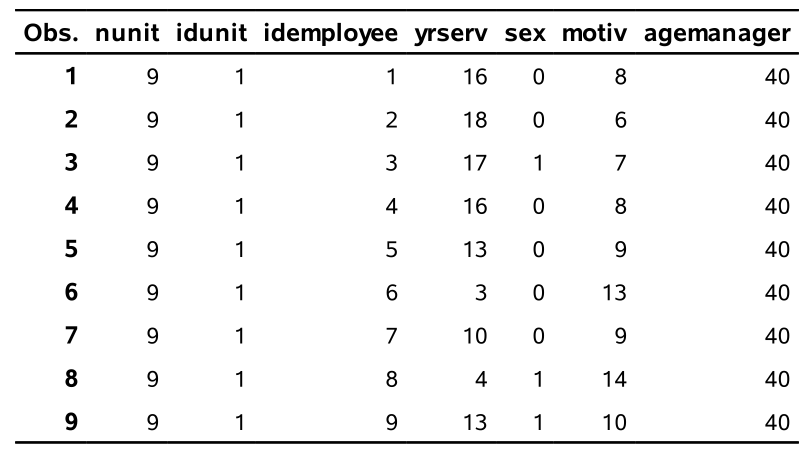
\includegraphics[width = 0.7\linewidth]{img/c6/slides7-e06}
\end{center}
{\small 
There are two types of variables, both of which can be included in the model: 
\be

\item those fixed for all individuals in the unit (\code{nunit} and \code{agemanager}) 
\item others that vary within unit (\code{yrserv} and \code{sex}). 
\ee
}
\end{frame}

\begin{frame}[fragile]
\frametitle{Grouping variable and study objective}
\bi
\item In the longitudinal \texttt{revenge} example, the group variable was the individual and we only had explanatory variables that were fixed for each person, i.e., fixed in time, with the exception of the time variable itself.
\item Here there are $100$ groups in total, and $1016$ observations in the file. 
\item The goal is to study the impact of sex, years of service, unit size, and of the age of the manager on worker mobilisation. 
\item However, we must account for the potential within-unit correlation. There is no natural ordering for the observations within a unit (contrary to the \texttt{revenge} example which contained repeated measurements over time).
\ei
\end{frame}


\begin{frame}[fragile]
\frametitle{Covariance structure for worker motivation}
\bi
\item We can consider the compound symmetry covariance structure to account for within-unit correlation. 
\bi

\item This means that we assume that the (conditional) correlation between a pair of observations in the same unit is always the same.
\ei
   
 \begin{tcolorbox}[colback=white, colframe=hecblue, title=\SASlang{} code for a linear model with equicorrelated errors]
 \begin{small}
\begin{verbatim}
proc mixed data=infe.motivation method=reml; 
class idunit; 
model motiv = sex yrserv agemanager nunit / solution; 
repeated / subject=idunit type=cs r=1 rcorr=1; 
run;
\end{verbatim}
\end{small}
\end{tcolorbox}
\ei
\end{frame}
% 
%  \begin{frame}
% \frametitle{Model specifications}
% \begin{center}
% \includegraphics[scale=0.5]{Figures/long75.pdf}
% \includegraphics[scale=0.5]{Figures/long76.pdf}\\
% \includegraphics[scale=0.5]{Figures/long78.pdf}
% \includegraphics[scale=0.5]{Figures/long79.pdf}\\
% \includegraphics[scale=0.5]{Figures/long77.pdf}
% \end{center}
% \end{frame}

 \begin{frame}
\frametitle{Covariance matrix within-unit (unit 1)}
\begin{center}
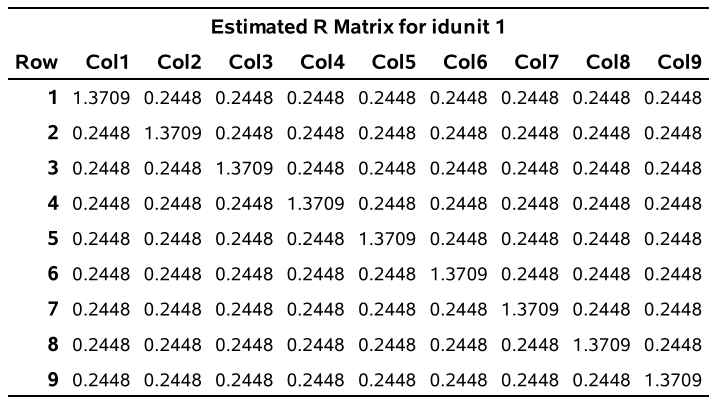
\includegraphics[width = 0.85\linewidth]{img/c6/slides7-e07}

\end{center}
\end{frame}

 \begin{frame}
\frametitle{Compound symmetry model}
\begin{center}
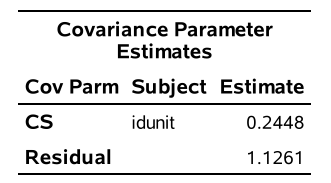
\includegraphics[width = 0.42\linewidth]{img/c6/slides7-e08}
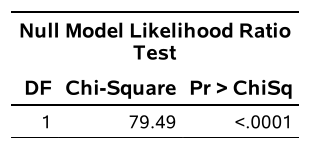
\includegraphics[width = 0.37\linewidth]{img/c6/slides7-e09}
\end{center}
\bi
\item The estimated covariance parameter from the compound symmetry model is $\hat{\tau} = 0.2448$. It is significantly different from $0$, suggesting a positive correlation between the worker motivation score between employees in the same unit, after adjusting for the effects of the explanatory variables. 
\item This estimated correlation between workers within-unit is $\hat{\rho} = 0.1785$. 
\ei
\end{frame}

% 
% \begin{frame}[fragile]
% \frametitle{Parameter coefficients as fixed effects}
% \bi
% \item  Consider the model we've used up to now:
% \begin{align*}
% Y_{ij}=\beta_0 + \beta_1 \mathrm{X}_{ij1}+\beta_2\mathrm{X}_{ij2}+\cdots+\beta_p\mathrm{X}_{ijp} + \varepsilon_{ij}
% \end{align*}
% for $i=1, \ldots, m$ and $j=1, \ldots, n_i$.
% \item In this model, $\bs{\beta}$ represent the \alert{fixed effects} which are the same for all individuals in the population. 
% \bi 
% \item The parameter $\beta_j$ describes how the mean of $Y$ varies as a function of $\mathrm{X}_j$ at the population level. 
% \ei
% 
% % \item The class of models for correlated data that we saw in the last section is a special case of a linear mixed model which we will outline soon.
% \ei
% \end{frame}

 \begin{frame}
\frametitle{Fixed effect estimates}
\begin{center}
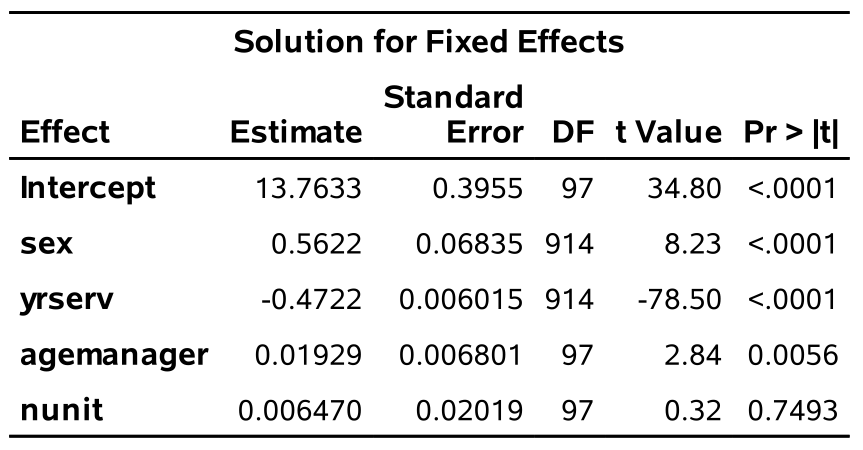
\includegraphics[width = 0.7\linewidth]{img/c6/slides7-e10}
\end{center}
\bi
\item The effects of three explanatory variables are significant: \code{sex}, \code{yrserv} and \code{agemanager}.
\bi

\item women are more motivated than men, on average. 
\item The longer a person has been employed at the company, the less (s)he is motivated. 
\item The older the manager, the more motivated the employee. 
\ei
\item However, the size of the unit is not significant.
\ei
\end{frame}


\begin{frame}[fragile]
\frametitle{Example: worker motivation}
\bi
\item It might be interesting to include an effect for the unit variable in the model. 
\item But, as we've already seen, when we include a fixed effect for each group, we lose the ability to estimate the effects of variables which are fixed within group. 
\item This would mean we could not include the variables \code{agemanager} or \code{nunit}.
\item However, there is still a way to include a ``group effect'' while also keeping the possibility of including variables which are fixed within group. 
\item We need to use \alert{random effects} instead of fixed effects, which can also be used to model the covariance structure.
\ei
\end{frame}

\begin{frame}[fragile]
\frametitle{Random effects models}
\bi
% \item  As mentioned earlier, mixed models allow us to include random effects. 
\item When an explanatory variable is modeled with a random effect, we assume that \alert{the total effect of this variable is a combination of}
\be

\item a \alert{common effect} for the entire population and  
\item a \alert{within-group effect}. 
\ee
\item For example, when considering repeated measures from the same individuals, the effect of a variable can be split into a common effect for all individuals in the population, and a unique effect for each individual. 
\item In the example of worker motivation, the effect of years of service could be split up into a common effect for all employees (in all units) and a unique effect in each unit for employees.
\ei
\end{frame}


% \begin{frame}[fragile]
% \frametitle{Random effects models}
% 
% 
% \end{frame}


\begin{frame}[fragile]
\frametitle{Random effects models}
\bi
\item The simplest random effects model is one with only a group-specific intercept, assumed random. 
\item The equation of the linear regression model is
\begin{align*}
Y_{ij}=\beta_0 + \beta_1 \mathrm{X}_{ij1}+\beta_2\mathrm{X}_{ij2}+\cdots+\beta_p\mathrm{X}_{ijp} + \varepsilon_{ij}
\end{align*}
for $i=1, \ldots, m$ and $j=1, \ldots, n_i$ and where $Y_{ij}$ is observation $j$ from group $i$.
\item Assume for now that the $\varepsilon_{ij} \simiid \Cn(0,\sigma^2)$. 
\item Suppose that we want to allow the intercept $\beta_0$ to vary from one group to another, but with a random effect.
\ei
\end{frame}


\begin{frame}[fragile]
\frametitle{Random effects models}
\bi
\item The model becomes
\begin{align*}
Y_{ij}=(\beta_0+b_i)+ \beta_1 \mathrm{X}_{ij1}+\beta_2\mathrm{X}_{ij2}+\cdots+\beta_p\mathrm{X}_{ijp} + \varepsilon_{ij}
\end{align*}
\item The \alert{intercept} \alert{specific to group $i$} is $\beta_0+b_i$. It consists of
\bi

\item A \alert{common effect over all groups}, $\beta_0$;
\item A \alert{group-specific effect}, $b_i$.
\ei 
\ei
\end{frame}

\begin{frame}[fragile]
\frametitle{Assumptions of the random intercept model}
The model equation is
\begin{align*}
Y_{ij}=(\beta_0+b_i)+ \beta_1 \mathrm{X}_{ij1}+\beta_2\mathrm{X}_{ij2}+\cdots+\beta_p\mathrm{X}_{ijp} + \varepsilon_{ij}
\end{align*}
\bi
\item The $b_1, \ldots, b_m$ quantities are assumed to be \alert{independent} random variables (and also independent from the $\varepsilon$ terms and the explanatory variables).
\item We assume both random intercepts and errors are normally distributed,
\bi \item $b_i\sim \Cn(0, \sigma^2_b)$ for all $i$ ($i=1, \ldots, m)$.
\item $\varepsilon_{ij}\sim \Cn(0, \sigma^2)$.
\ei
\item The $\varepsilon_{ij}$ terms could be correlated within group $i$, but they are assumed independent for the time being.
\ei
\end{frame}




\begin{frame}[fragile]
\frametitle{Random effects models: mean}
In this model, we still have the so-called \alert{marginal mean} of $Y_{ij}$,
\begin{align*}
\E{Y_{ij}\mid \mathbf{X}_i}=\beta_0+\beta_1\mathrm{X}_{ij1}+\beta_2\mathrm{X}_{ij2}+\cdots + \beta_p\mathrm{X}_{ijp}.
\end{align*}
\bi
\item At the population level, the mean of $Y_{ij}$ is only a function of the fixed effects. 
\ei
We also have the \alert{conditional mean} of $Y_{ij}$, which depends on the group-specific effect,
\begin{align*}
\E{Y_{ij}\mid \mathbf{X}_i, b_i}=\beta_0+b_i+\beta_1\mathrm{X}_{ij1}+\beta_2\mathrm{X}_{ij2}+\cdots + \beta_p\mathrm{X}_{ijp}
\end{align*}
\bi
\item It is possible to get predicted values for the random variables $b_i$.
\ei
\end{frame}


\begin{frame}[fragile]
\frametitle{Random effects models}
\bi
\item With this kind of model, we can estimate the mean $\E{Y_{ij}\mid \mathbf{X}_i, b_i}$  which can be thought of as a \alert{prediction} of the value of $Y_{ij}$ after accounting for the group-specific effects. 
\item In repeated measures data, this allows us to predict an individual's trajectory
while accounting for specific effects of the individual.
\item One interesting fact is that when we add a random effect for the group variable, we can still estimate effects of variables that are fixed within a group.
\ei
\end{frame}


\begin{frame}[fragile]
\frametitle{Random effects models: variance/covariance}

Since it's random, the term $b_i$ introduces a \alert{within-group correlation in the model}. Because $\eps_{ij}$ is independent of $b_i$ for all $i, j$, the (conditional) variance of an observation is
\begin{align*}
\Va{Y_{ij}\mid \mathbf{X}_i}&=\Va{b_i}+\Va{\varepsilon_{ij}}=\sigma^2_b + \sigma^2_{\vphantom{b}}
\end{align*}
The covariance between two individuals in the same group is
\begin{align*}
\Co{Y_{ij}, Y_{ik}\mid \mathbf{X}_i}=\sigma^2_b, \qquad j\neq k.
\end{align*}
Consequently, the correlation between two individuals in the same group is
\begin{align*}
\Cor{Y_{ij}, Y_{ik}\mid \mathbf{X}_i}=\frac{\sigma^2_b}{\sigma^2_{\vphantom{b}}+\sigma^2_b}, \qquad  j\neq k.
\end{align*}
This quantity is often called the \alert{intra-class correlation}.

\end{frame}
\begin{frame}{Mathematical aside}
Both  $\beta_j$ and explanatories are assumed non-random, thus
 \begin{align*}
  \Co{Y_{ij}, Y_{ik} \mid \mathbf{X}_i} &= \mathsf{Co}\left(\beta_0 +b_i + \beta_1\mathrm{X}_{ij1}+\cdots + \eps_{ij},\right.\\
  & \quad \qquad \left.\beta_0 +b_i + \beta_1\mathrm{X}_{ik1}+\cdots + \eps_{ik} \mid \mathbf{X}_i\right)
  \\&= \Co{b_i+ \eps_{ij}, b_i + \eps_{ik}}
  \\&= \Va{b_i} + \Co{\eps_{ij}, \eps_{ik}} = \sigma^2_b.
\end{align*}
where the last step follows from independence of $b_i$ and $\eps$'s and because $\Co{Y_{ij},Y_{ij}}=\Va{Y_{ij}}$.

\end{frame}
\begin{frame}{Variability of $\bs{Y}$}


Alternatively,
\begin{align*}
   \Va{\bs{Y}_i \mid \mathbf{X}_i} &= \Va{
   \begin{matrix} b_i \\ \vdots \\ b_i 
   \end{matrix}
   } + \Va{\begin{matrix}\eps_{i1} \\ \vdots \\ \eps_{in_i}\end{matrix}} \\&= 
   \begin{pmatrix}
 \sigma^2_b &  \sigma^2_b & \cdots & \sigma^2_b \\
  \sigma^2_b &  \sigma^2_b & \cdots & \sigma^2_b \\
 \vdots & \ddots & \ddots & \vdots \\
 \sigma^2_b &  \sigma^2_b & \cdots & \sigma^2_b   
 \end{pmatrix} + \begin{pmatrix}
 \sigma^2 & 0 & \cdots &0\\
 0 & \sigma^2 & \ddots &0\\
 \vdots &\ddots & \ddots & \vdots\\
 0 & 0 & \cdots & \sigma^2
 \end{pmatrix}.
\end{align*}

\end{frame}


\begin{frame}[fragile]
\frametitle{Compound symmetry correlation induced by the random intercept model}
\bi
\item We can see that introducing a random effect for the intercept implies that the observations within the same group are correlated, and the correlation is the same regardless of which individuals are considered (equicorrelation).
\item The difference is that now the correlation must be non-negative, since $\sigma^2_b$ is a variance whereas the correlation for the compound symmetry model was \[-\frac{1}{\max(n_i)+1} \leq \rho \leq 1.\]
\item This limitation is not usually of consequence, because within-group correlations tend to be positive.
\item \textbf{Adding a random intercept is the same as using the compound symmetry structure.}

\ei
\end{frame}


\begin{frame}[fragile]
\frametitle{Adding a random intercept with the \code{random} command} 
\bi 
\item The command \code{repeated} allows us to specify the covariance structure for the errors in \code{proc mixed}. 
\item If we don't use the \texttt{repeated} command, the errors are assumed to be independent.
\ei
\begin{tcolorbox}[colback=white, colframe=hecblue, title=\SASlang{} code for a random intercept model with independent errors]
\begin{small}
\begin{verbatim}
proc mixed data=infe.motivation; 
class idunit; 
model motiv = sex yrserv agemanager nunit / solution; 
random intercept / subject=idunit v=1 vcorr=1; 
run;
\end{verbatim}
\end{small}
\end{tcolorbox}
{ \footnotesize   Including a random intercept \alert{naturally} induces a compound symmetry correlation structure.
Therefore, we do not need to specify anything for the covariance structure of the errors.


}
\end{frame}
% 
% \begin{frame}[fragile]
% \frametitle{Remarks on the \SASlang{} code}
% \bi
% \item It's important to note that we have not assumed any structure on the covariance of the errors here --- there is no \texttt{repeated} command in the \SASlang{} code.
% \item As we've already seen, including a random intercept \alert{naturally} induces a compound symmetry correlation structure.
% \item Therefore, we do not need to specify anything for the covariance structure of the errors.
% \ei
% \end{frame}
% 
% \begin{frame}[fragile]
% \frametitle{Model specification}
% \begin{center}
% \includegraphics[scale=0.5]{Figures/long88.pdf}
% \end{center}
% \end{frame}

\begin{frame}[fragile]
\frametitle{Covariance matrix specified by the random intercept model}
\begin{center}
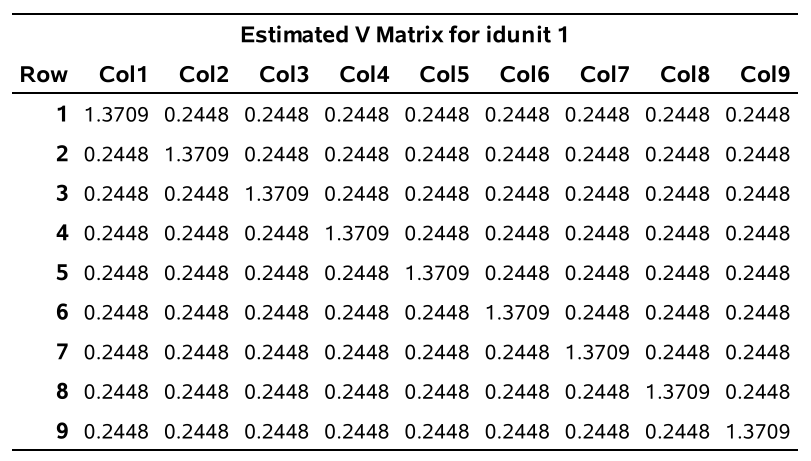
\includegraphics[width = 0.9\linewidth]{img/c6/slides7-e11}

\end{center}
\end{frame}

% \begin{frame}[fragile]
% \frametitle{Correlation matrix for the data}
% \begin{center}
% 
% \end{center}
% \end{frame}

\begin{frame}[fragile]
\frametitle{Covariance parameter estimates}
\begin{center}
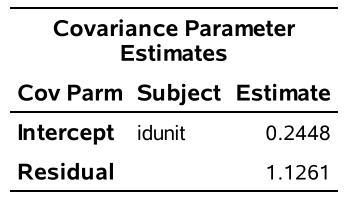
\includegraphics[width = 0.4\linewidth]{img/c6/slides7-e12}
\end{center}
\bi
\item The variance estimate for the random intercept is
$\hat{\sigma}^2_b=0.2448$, whereas the estimate of the variance of the error term is
$\hat{\sigma}^2= 1.1261$.
\item Consequently, the estimate of the within-unit correlation is
\begin{align*}
\hat{\rho}=\frac{\hat{\sigma}^2_b}{\hat{\sigma}^2_b+\sigma^2_{\vphantom{b}}}=0.1785.
\end{align*}
% \item This agrees with the value reported in the correlation matrix for individual 1. 
\item This is exactly the same correlation for the observation than that obtained from compound symmetry covariance model for the errors (command \code{repeated}).
\ei
\end{frame}

\begin{frame}[fragile]
\frametitle{Fixed effect estimates}
\begin{center}
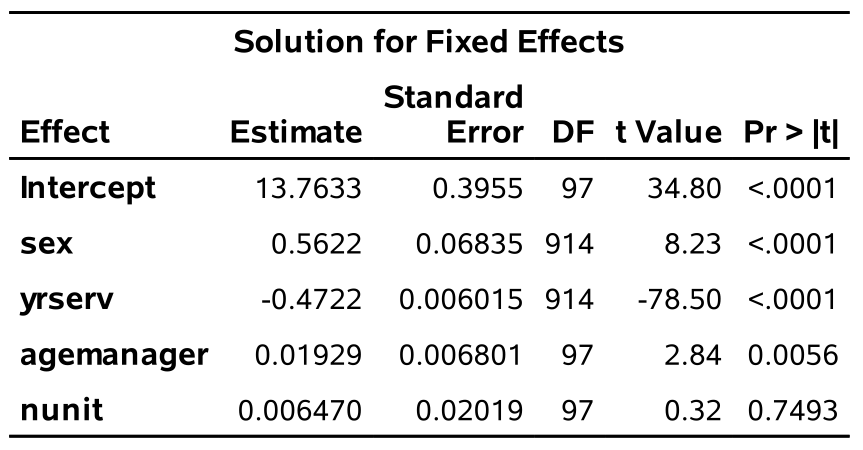
\includegraphics[width = 0.7\linewidth]{img/c6/slides7-e10}
\end{center}
{\footnotesize The effects of the explanatory variables (and their standard errors)
are also the same as for the compound symmetry structure --- both models are equivalent for the response assuming the within-unit correlation is positive. 


}
\end{frame}
% 
% \begin{frame}[fragile]
% \frametitle{Random effects models}
% \bi
% \item Using a random intercept is equivalent to using a compound symmetry structure (assuming the intra-class correlation is positive).
% \item In general, the two approaches are different.
% \ei
% \end{frame}
% 

 \begin{frame}
\frametitle{Longitudinal data}
\bi
\item In the worker motivation example, the natural correlation structure for the data is the equicorrelation  structure, which assumes that each pair of observations within a group has the same correlation, because the groups represent units in a company.
\item We've seen that it's not necessary to model the covariance structure by assuming a structure on the errors  of the model; we just need to include a random intercept which will automatically induce a compound symmetry structure on the data. 
\item However, this kind of structure might not be valid in longitudinal data, and we might want to use an $\mathsf{AR}(1)$ structure, as we saw in the customer revenge example.
\ei
\end{frame}

 \begin{frame}
\frametitle{Longitudinal data}
\bi
\item In longitudinal data, specifying an $\mathsf{AR}(1)$ structure for the data can be done by adding a structure on the errors of the data, \alert{as well as through the specification of random effects}.
\item The model is
\begin{align*}
Y_{ij}=\beta_0 +b_i + \beta_1 \mathrm{X}_{ij1}+\beta_2\mathrm{X}_{ij2}+\cdots+\beta_p\mathrm{X}_{ijp} + \varepsilon_{ij}
\end{align*}
but we now assume 
\bi

\item for the random intercept term, $b_{i} \simiid \Cn(0, \sigma^2_b)$,
\item  for the errors, $\bs{\varepsilon}_i \sim \Cn\big(\bs{0}_{n_i}, \bs{\Sigma}_i\big)$,
\item $\varepsilon_{ij}$ are \alert{not independent} within each subject $i$ --- $\bs{\Sigma}_i$ is not diagonal.
\ei
\item We can assume an $\mathsf{AR}(1)$ structure (or a structure other than compound symmetry) on the covariance matrix of the errors $\bs{\Sigma}_i$.
\ei

{\footnotesize Side remark:
 while the matrices $\bs{\Sigma}_i$ may share the same parameter values for each subject $i$, they need not be the same size, hence the subscript.
 
 }
\end{frame}
 
\begin{frame}[fragile]
\frametitle{Random intercept with $\mathsf{AR}(1)$ structure}
\begin{tcolorbox}[colback=white, colframe=hecblue, title=\SASlang{} code for the random intercept model with $\mathsf{AR}(1)$ errors]
\begin{verbatim}
proc mixed data=revenge; 
class id tcat; 
model revenge = sex age vc wom t / solution;
random intercept / subject=id v=1 vcorr=1; 
repeated tcat / subject=id type=ar(1) r=1 rcorr=1;
run;
\end{verbatim}
\end{tcolorbox}

\bi
\item The option \texttt{v=1 vcorr=1} tells \SASlang{} to output the covariance/correlation matrix for the \alert{$\bs{Y}$ observations} for subject $1$.
\item The option \texttt{r=1 rcorr=1}  tells \SASlang{} to output the covariance/correlation matrix for the \alert{errors $\bs{\varepsilon}$} for subject $1$.
\ei
\end{frame}

\begin{frame}[fragile]
\frametitle{Covariance and correlation matrices for the \textbf{errors}}
\begin{center}
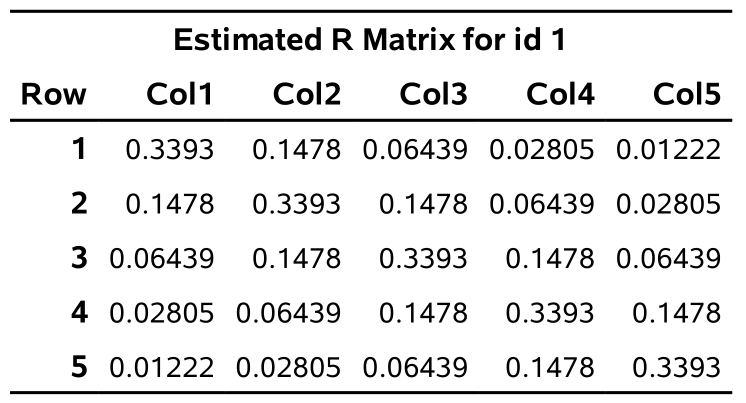
\includegraphics[width=0.49\linewidth]{img/c6/slides7-e13}
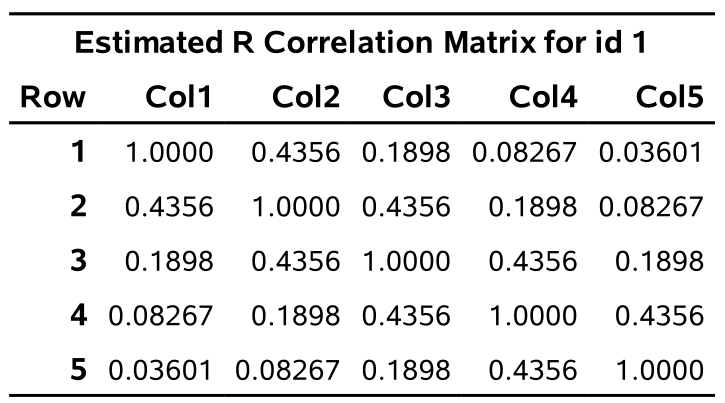
\includegraphics[width=0.48\linewidth]{img/c6/slides7-e14}
\end{center}

\end{frame}

\begin{frame}[fragile]
\frametitle{Covariance and correlation matrices for the \textbf{observations}}
\begin{center}
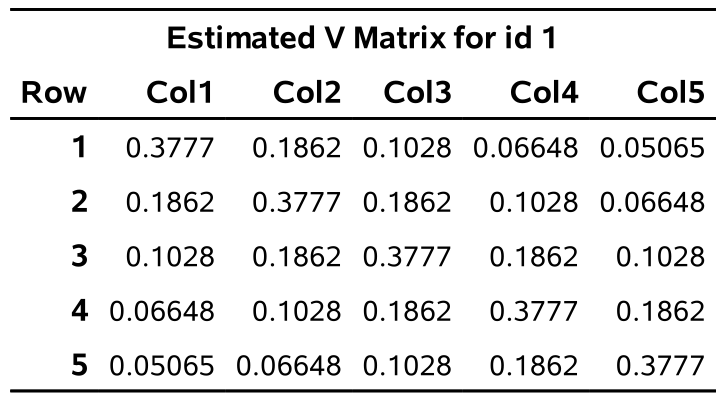
\includegraphics[width=0.50\linewidth]{img/c6/slides7-e15}
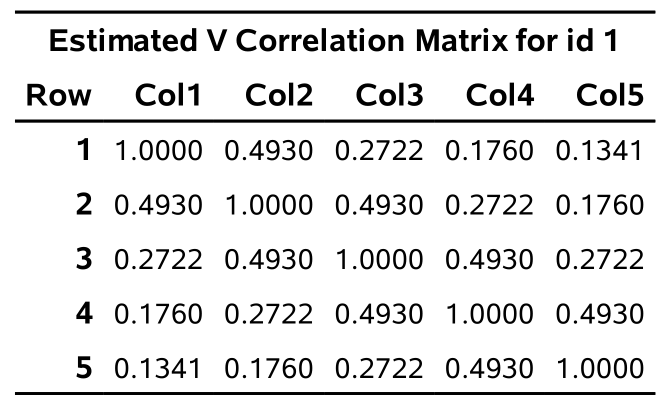
\includegraphics[width=0.46\linewidth]{img/c6/slides7-e16}
\end{center}
\bi
\item Note that these matrices are different than the ones for the errors in the previous slide.
\item The covariance of the \alert{data} is the sum of that of the random effects and of the covariance on the errors.
\ei
\end{frame}


% \begin{frame}[fragile]
% \frametitle{Covariance parameters}
% \begin{center}
% \includegraphics[scale=0.8]{Figures/long123_5.pdf}
% \end{center}
% There are three covariance parameters in the model:
% \bi
% \item The variance of the random effect $\hat{\sigma}^2_b=0.038$ (not significant). 
% \bi \item[] \textbf{warning: non-regular test, unreliable output!}\ei
% \item The variance of the residuals $\varepsilon$, $\hat{\sigma}^2_e$, is $0.33$.
% \item The lag-one correlation $\hat{\rho}=0.43$ of the $\mathsf{AR}(1)$ model (significant).
% \ei
% \end{frame}
\begin{frame}[fragile]
\frametitle{Covariance parameters}
\begin{center}
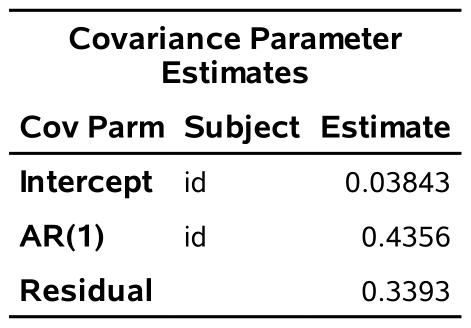
\includegraphics[width = 0.4\linewidth]{img/c6/slides7-e17}
\end{center}
There are three covariance parameters in the model, the estimates of which are 
\bi
\item $\hat{\sigma}^2_b=0.038$ for the variance of the random effect, 
\item $\hat{\sigma}^2=0.33$ for the variance of the errors $\varepsilon$, 
\item $\hat{\rho}=0.43$ for the lag-one correlation of the $\mathsf{AR}(1)$ model.
\ei
\end{frame}
\begin{frame}[fragile]
\frametitle{Information criteria and fixed effects}
\begin{center}
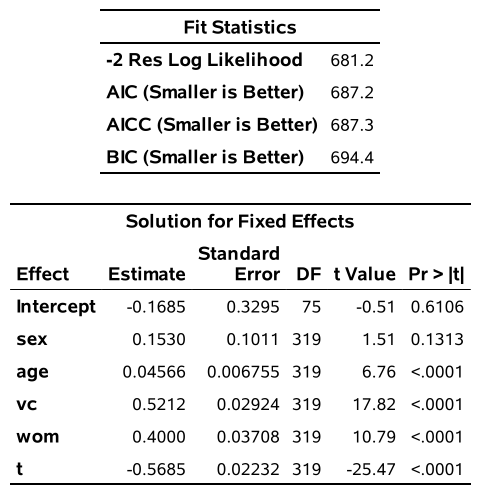
\includegraphics[width =0.6\linewidth]{img/c6/slides7-e18}
\end{center}
{\footnotesize 
These estimates are for the mixed model with a random intercept for \texttt{id} and an $\mathsf{AR}(1)$ structure for the errors. We can compare it using information criteria to the model that includes does not include the random intercept from Chapter 6.

}
\end{frame}


% \begin{frame}[fragile]
% \frametitle{Investigation of the usefulness of the random intercept}
% \bi
% \item Testing whether the variance of the random effect $\sigma^2_b=0$ (corresponding to no random intercept) is a non-standard testing problem \ldots 
% \item The model which includes a random intercept and an $\mathsf{AR}(1)$ covariance structure within-unit for the residuals had a $\mathsf{BIC}$ ($\mathsf{AIC}$) of $694.4$ ($687.2$) compared to $690.5$ ($685.8$) for the model that assumes independent residuals.
% \item According to the $\mathsf{BIC}$, the best model is the one without a random effect, but with an $\mathsf{AR}(1)$ correlation on the errors. $\mathsf{AIC}$ prefers more complicated models and so includes the random intercept.
% \item It seems that modelling an intercept for each subject is not necessary in this example. The $\mathsf{AR}(1)$ correlation of the errors appears to be sufficient in explaining the correlation in the data.
% \ei
% \end{frame}
\begin{frame}
 \frametitle{Fixed or random effect?}
 \bi \item The theory we cover generalizes to more complex setting (e.g., we could allow random slopes for each groups).
 \item Loosely speaking, the main difference between fixed and random effects is 
 \bi 
%  \item At the population level, we assume that the average random effect is zero (or else captured by a fixed effect coefficient).
 \item \textbf{fixed effects} for group are used when we have few groups and lots of replicates and we care about the effect of the group (small $m$, large $n_i$).
 \item \textbf{random effects} are used when there are enough levels of the factor group to estimate the variance $\sigma^2_b$ reliably; we are not interested in the effects per say (large $m$, small $n_i$).
 \ei
 \item Testing whether a random effect is needed or not is equivalent to testing if the variance of the random effect $\sigma^2_b=0$; this is a non-standard testing problem, which is beyond the scope of this course\ldots 
 \ei
\end{frame}

% 
% \begin{frame}
% \frametitle{Chapter overview}
% 
% 
% \begin{tcolorbox}[colback=white, colframe=hecblue, title=Chapter 7 - Models for longitudinal and correlated data]
% \bi
% 
% \begin{tiny}
% \item[1.] Introduction and example
% \item[2.] Covariance and correlation matrix
% \item[3.] Linear model with correlated errors
% \item[4.] Choice of covariance structure
% \item[5.] Hypothesis testing on the covariance structure
% \item[6.]  Linear model with correlated errors and a group effect
% \item[7.] Random intercept model
% \item[8.]  \textbf{\alert{Random slope model}}
% \item[9.] Prediction
% \item[10.] Example of a model with a more complex covariance structure
% \end{tiny}
% \ei
% \end{tcolorbox}
% \end{frame}



%  \begin{frame}
% \frametitle{Random effects on the predictor variables}
% \bi
% \item In the last section, we saw that it's possible to incorporate a within-group correlation through random effects, but we limited ourselves to models with only a random intercept. 
% \item We will now consider the general case of a random effect, where a random effect can be included for any of the explanatory variables. 
% \ei
% \end{frame}


% \begin{frame}
% \frametitle{Random effects on the predictor variables}
% \bi
% \item Let's revisit the linear regression model for correlated data,
% \begin{align*}
% Y_{ij}=\beta_0 +b_i + \beta_1 \mathrm{X}_{ij1}+\beta_2\mathrm{X}_{ij2}+\cdots+\beta_p\mathrm{X}_{ijp} + \varepsilon_{ij},
% \end{align*}
% where we again assume independence of $\varepsilon_{ij} \simiid \Cn(0, \sigma^2)$.
% \item Assume that, in addition to the intercept, the effect of the first predictor $X_1$ is random, i.e.,
% \begin{align*}
% Y_{ij}=(\beta_0 +\alert{b_i}) + (\beta_1+\alert{b_{1i}})X_{ij1}+\beta_2\mathrm{X}_{ij2}+\cdots+\beta_p\mathrm{X}_{ijp} + \varepsilon_{ij}.
% \end{align*}
% 
% \ei
% \end{frame}
% 
% 
% 
% 
% 
% \begin{frame}
% \frametitle{Random effects on the predictor variables}
% The model equation is
% \begin{align*}
% Y_{ij}=(\beta_0 +\alert{b_i}) + (\beta_1+\alert{b_{1i}})X_{ij1}+\beta_2\mathrm{X}_{ij2}+\cdots+\beta_p\mathrm{X}_{ijp} + \varepsilon_{ij}.
% \end{align*}
% 
% \bi
% \item The effect of the variable $X_1$ \alert{for group $i$} is then $\beta_1 + b_{1i}$
% \item Just like in the random intercept model we saw in the last section, 
% the effect of $X_1$ includes an effect common to all groups, $\beta_1$ , and a group-specific effect, $b_{1i}$. 
% \item The parameter $\beta_1$ is the effect (slope) of $X_1$ \alert{averaged over the entire population} 
% \item $\beta_1+b_{1i}$ is the effect of $X_1$ \alert{specific to group
% $i$}.
% \ei
% \end{frame}
% 
% \begin{frame}
% \frametitle{Model assumptions}
% \begin{align*}
% Y_{ij}=(\beta_0 +\alert{b_i}) + (\beta_1+\alert{b_{1i}})X_{ij1}+\beta_2\mathrm{X}_{ij2}+\cdots+\beta_p\mathrm{X}_{ijp} + \varepsilon_{ij}.
% \end{align*}
% \bi
% \item The random effects follow 
% \[
% \begin{pmatrix}
%  b_i\\ b_{1i}
% \end{pmatrix} \sim \Cn_2 \left[ \begin{pmatrix}
% 0 \\ 0
% \end{pmatrix},   \begin{pmatrix}
%     \sigma_{b_0}^2 & \sigma_{b01}  \\
%     \sigma_{b01} & \sigma_{b_1}^2  \\
%   \end{pmatrix}\right].
% \]
% \item We assume as before that $\varepsilon_{ij}\sim \Cn(0, \sigma^2_{\varepsilon})$.
% \item The $\varepsilon_{ij}$ could also be correlated within group $i$. 
% \ei
% \end{frame}


\begin{frame}
\frametitle{Conditional and marginal means}
\bi
\item At the population level, the marginal mean of $Y_{ij}$ is, as usual,
\begin{align*}
\E{Y_{ij}\mid \mathbf{X}_i}=\beta_0  + \beta_1 \mathrm{X}_{ij1}+\beta_2\mathrm{X}_{ij2}+\cdots+\beta_p\mathrm{X}_{ijp}.
\end{align*}
\item However, the \alert{conditional mean} of $Y_{ij}$, given by the group specific effects, is
\begin{align*}
\E{Y_{ij}\mid \mathbf{X}_i, b_i}&=(\beta_0 + \alert{b_i}) + \beta_1 \mathrm{X}_{ij1}+\cdots+\beta_p\mathrm{X}_{ijp}.
\end{align*}
\item By predicting the random effect $b_i$, we can predict the value of $Y_{ij}$ while accounting for the group-specific random effect for the intercept.
\ei
\end{frame}

\begin{frame}[fragile]
\frametitle{Graphical illustration}
We can display the random intercept for the \texttt{revenge} data. Both models are fitted with $\mathsf{AR}(1)$ covariance for the errors and \texttt{t} as fixed effect.

\begin{center}
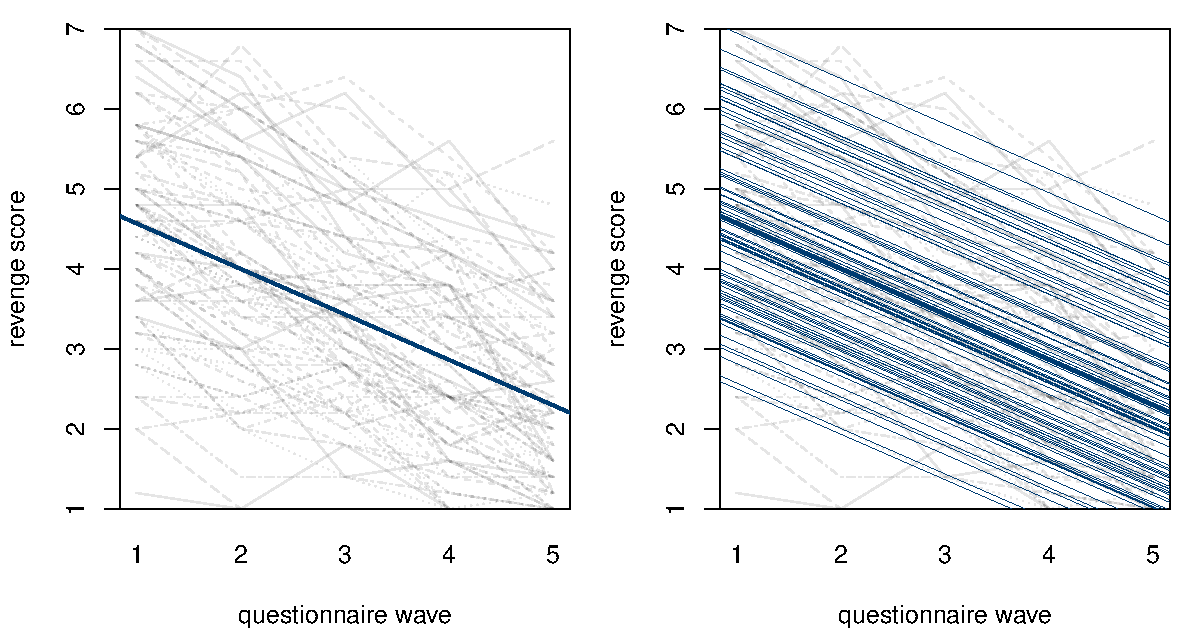
\includegraphics[width = 0.8\linewidth]{img/c6/07-mixed-randomintercept}
\end{center}
{\footnotesize 
Model without (left) and with random intercept for \texttt{id} (right).

}
\end{frame}
% 
% \begin{frame}
% \frametitle{Variance/covariance of the data}
% \bi
% \item \textbf{Including a random effect for a predictor variable
% means that the covariance matrix of $Y_{ij}$ depends on this predictor variable.} 
% \item The variance of $Y_{ij}$ induced by the random effects is
% \begin{align*}
% \Va{Y_{ij}\mid    _i}=\sigma_{b_0}^2+X_{ij1}^2 \sigma_{b_0}^2 + 2\mathrm{X}_{ij1} \sigma_{b01}+\sigma^2_{\varepsilon}.
% \end{align*}
% \item If we assume that the residuals are independent, the covariance between two observations in the same group $(j\neq k)$ is
% \begin{align*}
% \Co{Y_{ij}, Y_{ik}\mid \mathbf{X}_i}=\sigma^2_{b_0}+X_{ij1}X_{1ik}\sigma^2_{b_1}+(X_{ij1}+X_{1ik})\sigma_{b01}.
% \end{align*}
% \item If we add structure to the covariance of the residuals, then the covariance of the observations is more complex\ldots 
% 
% \ei
% \end{frame}
% 
% \begin{frame}[fragile]
% \frametitle{Example model with random intercept}
% Using the worker motivation data, we fit a model with a random intercept as well as a random effect for \code{yrserv} (years of service). 
% 
% 
% \begin{tcolorbox}[colback=white, colframe=hecblue, title=\SASlang{} code for random intercept model]
% \begin{verbatim}
% proc mixed data=infe.longitud3 ;
% class idunit;
% model motiv = sex yrserv agemanager nunit 
%       / solution;
% random intercept yrserv /subject=idunit v1= vcorr=1;
% run;
% \end{verbatim}
% \end{tcolorbox}
% \end{frame}
% 
% \begin{frame}
% \frametitle{\SASlang{} output}
% \textbf{Correlation matrix for the data}
% \begin{center}
% \includegraphics[scale=0.45]{Figures/long122_1.pdf}%
% \includegraphics[scale=0.45]{Figures/long122_2.pdf}
% \end{center}
% \bi
% \item The correlation between pairs of observations is not constant.
% \item This correlation depends on the values of the covariates.
% \item In this case, there are covariates that are not fixed within group.
% \ei
% \end{frame}
% 
%  \begin{frame}
% \frametitle{Covariance parameters}
% \begin{center}
% \includegraphics[width = 0.4\linewidth]{Figures/cov11}
% \end{center}
% \bi
% \item There are three estimated covariance parameters in the model:
% \bi
% \item The variance of the random intercept is $\hat{\sigma}_{b_0}^2=0.16$.
% \item The variance of the random effect for \code{yrserv} is  $\hat{\sigma}_{b_1}^2=0.0008$.
% \item The variance of the residuals (assumed independent ) is $\hat{\sigma}^2_{\varepsilon}=1.09$.
% \ei
% \ei
% \end{frame}
% 
%  \begin{frame}
% \frametitle{AIC, BIC and fixed effects}
% \begin{center}
% \includegraphics[scale=0.6]{Figures/long122_4.pdf}
% \includegraphics[scale=0.6]{Figures/long122_5.pdf}
% \end{center}
% \bi
% \item The BIC for the model with only a random intercept was 3152.3. Now it's 3148.9. It appears that the model with a unit-specific effect for \texttt{yrserv} is more appropriate.
% \ei
% \end{frame}


% \begin{frame}
%\frametitle{Exercice: sortie \SASlang{}}
%\begin{center}
%\includegraphics[scale=0.6]{Figures/ex9.pdf}
%\includegraphics[scale=0.6]{Figures/ex10.pdf}\\
%\includegraphics[scale=0.6]{Figures/ex11.pdf}
%\includegraphics[scale=0.6]{Figures/ex12.pdf}
%\end{center}
%\end{frame}
%
% \begin{frame}
%\frametitle{Exercice: sortie \SASlang{}}
%\begin{center}
%\includegraphics[scale=0.6]{Figures/ex13.pdf}
%\end{center}
%\end{frame}


% \begin{frame}
% \frametitle{Chapter overview}
% 
% 
% \begin{tcolorbox}[colback=white, colframe=hecblue, title=Chapter 7 - Models for longitudinal and correlated data]
% \bi
% 
% \begin{tiny}
% \item[1.] Introduction and example
% \item[2.] Covariance and correlation matrix
% \item[3.] Linear model with correlated errors
% \item[4.] Choice of covariance structure
% \item[5.] Hypothesis testing on the covariance structure
% \item[6.]  Linear model with correlated errors and a group effect
% \item[7.] Random intercept model
% \item[8.]  Random slope model
% \item[9.] \textbf{\alert{Prediction}}
% \item[10.] Example of a model with a more complex covariance structure
% \end{tiny}
% \ei
% \end{tcolorbox}
% \end{frame}
\section{Prediction for mixed effect models}
\begin{frame}
\frametitle{Prediction}
\bi
\item According to the model specification presented in the last section, the terms, $\bs{b}$, are \alert{random variables} and not parameters (i.e., fixed quantities but unknown). 
\item We can always get \alert{predictions} for these random variables. 
\item Be careful to not confuse \alert{prediction} with \alert{estimation}. Prediction is for random variables. 

\item Once we have predicted values for the $\bs{b}$ terms and estimates for the fixed effect parameters, $\beta$, we can get predictions for the outcome variables $\bs{Y}$. 
\ei
\end{frame}


\begin{frame}
\frametitle{Prediction: model \textbf{without} random effects}
\bi
\item \alert{If there are no random effects in the model} (for example, if we had fitted a model that directly specified the covariance structure using \code{repeated}), then we make predictions in the same way as we did for ordinary linear regression. 
\item That is, the prediction for $Y_{ij}$ is
\begin{align*}
\hat{Y}_{ij}=\hat{\beta}_0 + \hat{\beta}_1\mathrm{X}_{ij1} + \ldots + \hat{\beta}_p\mathrm{X}_{ijp}.
\end{align*}
\item This quantity is also the estimate of the \alert{mean} (at the \alert{population level}) of the response variable.
\ei
\end{frame}

\begin{frame}
\frametitle{Prediction: model \textbf{with} random effect}
\bi
\item If there are random effects in the model, the estimation of the \alert{mean} (at the \alert{population level}) of the response variable for an individual with the characteristics of individual $j$ from group $i$ is
\begin{align*}
\hat{Y}_{ij}=\hat{\beta}_0 + \hat{\beta}_1\mathrm{X}_{ij1} + \ldots + \hat{\beta}_p\mathrm{X}_{ijp}.
\end{align*}


\item But we can also get predictions of the
values of the response variable for individual $j$ in group $i$
\item For example, in a model with a random intercept $b_{i}$,
 \begin{align*}
\hat{Y}_{ij}=\hat{\beta}_0 +\hat{b}_{i} + \hat{\beta}_1\mathrm{X}_{ij1} + \ldots + \hat{\beta}_p\mathrm{X}_{ijp}. 
\end{align*}

\item If, however, we want to get predictions for a \alert{new}
individual that was not included in the original dataset, then we have no choice but to use the mean prediction, because the random effect estimate of this group is not available.
\ei
\end{frame}

\begin{frame}[fragile]
\frametitle{Predictions for random effects}
Let's revisit the last model for this example, with a random intercept.
\begin{tcolorbox}[colback=white, colframe=hecblue, title=\SASlang{} code for the random intercept model]
\begin{small}
\begin{verbatim}
proc mixed data=infe.motivation;
class idunit;
model motiv = sex yrserv agemanager nunit / solution;
random intercept / subject=idunit type=vc solution;
ods output Mixed.SolutionR=re;
run;
\end{verbatim}
\end{small}
\end{tcolorbox}
\begin{small} The option \code{solution} in the command \code{random} is used to get predictions of the random effects. The command \code{ods output}
saves these in order to make diagnostic plots for the random effets.\end{small}
\end{frame}

\begin{frame}
\frametitle{Predictions of the random effects}
\begin{center}
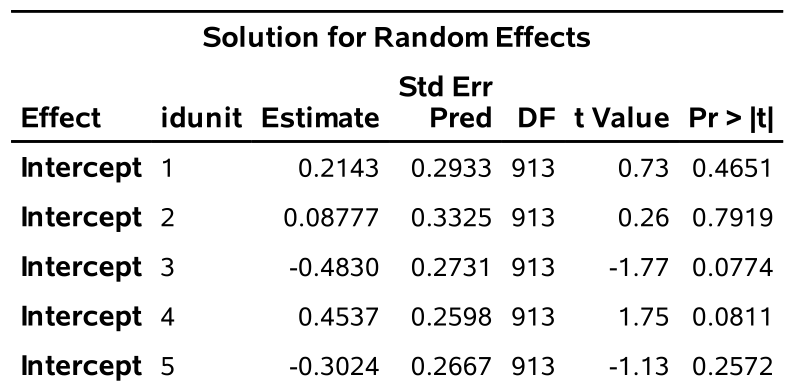
\includegraphics[width = 0.7\linewidth]{img/c6/slides7-e19}
\begin{align*}
 \vdots
\end{align*}
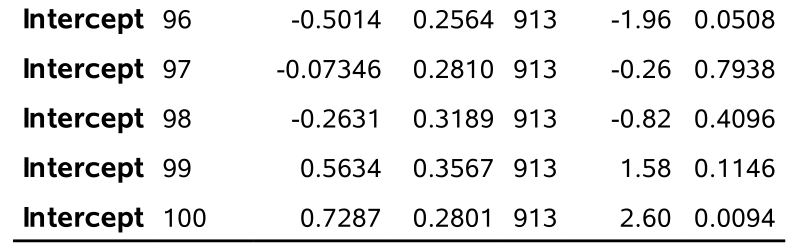
\includegraphics[width = 0.7\linewidth]{img/c6/slides7-e20}
\end{center}
\end{frame}

% \begin{frame}
% \frametitle{Predictions for the random effect terms of the first three units} 
% 
% \begin{center}
% \includegraphics[scale=0.5]{Figures/long118.pdf}
% \end{center}
% \begin{small} Only part of the table is shown here: the full table includes predictions for all $100$ units in the dataset. \end{small}
% \end{frame}
% 
\begin{frame}
\frametitle{Histogram of random effects}
We can plot histograms and quantile-quantile plots of the predicted random intercepts.
\begin{center}
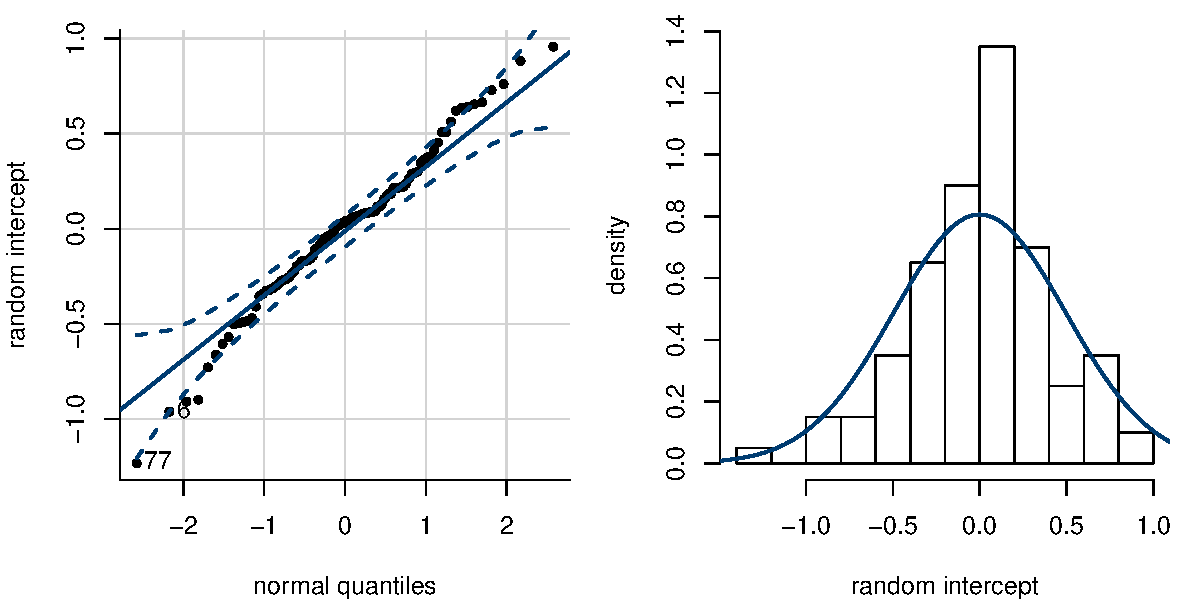
\includegraphics[width = 0.8 \linewidth]{img/c6/07-mixed-diagran.pdf}
% \includegraphics[width = 0.45 \linewidth]{Figures/long120.pdf}
\end{center}
These can help us check the normality assumption of the random effects (think of these as further residual diagnostics). Note that (by construction), the average of these random effects is always zero.
\end{frame}

% \begin{frame}
% \frametitle{Scatterplot of the random intercept $b_i$ as a function of $b_{1i}$}
% 
% \begin{center}
% \includegraphics[scale=0.35]{Figures/long121.pdf}
% \end{center}
% \bi
% \item We assumed that the two effects are independent. 
% \item This assumption can be relaxed in \code{proc mixed} by setting, e.g., \code{type = un}.
% \ei
% \end{frame}

\begin{frame}[fragile]
\frametitle{Predictions for observations $Y$}
\bi
\item With \code{\code{proc mixed}}, we can save the values \alert{for all observations in the data file}:
\bi
\item Predictions for the mean of the population (fixed effects),
\item Individual predictions (fixed and random effects).
\ei
\item This is done using the options \code{outpm}
and \code{outp}, respectively, in the \code{model} command.
\item \textbf{Trick}: If you want predictions for new individuals, you can just include these observations in the data file, while leaving the $Y$ variable blank (with ``.'' in \SASlang{}). These individuals will not be used in estimation of the model, but we will retrieve their predicted values.
\ei
\end{frame}

\begin{frame}[fragile]
\frametitle{Prediction for new employees}
We assume that we want to get predictions for two new employees, one of whom is part of a unit already present in the dataset (\code{idunit=1}) and one that is part of a unit not in the original dataset (\code{idunit=101}). 


\begin{tcolorbox}[colback=white, colframe=hecblue, title=\SASlang{} code to input two new observations]
\begin{small}
\begin{verbatim}
data newdata; 
input nunit idunit idemployee yrserv sex 
     motiv agemanager; 
cards; 
9 1 10 5 0 . 40 
9 101 1 5 0 . 40; 
run; 

/* Merge observations with database */
data motivation; 
set infe.motivation newdata; 
run;
\end{verbatim}
\end{small}
\end{tcolorbox}
\end{frame}

\begin{frame}[fragile]
\frametitle{Code to fit the model and get predictions}
\begin{tcolorbox}[colback=white, colframe=hecblue, title=\SASlang{} code to output predictions from a mixed model]
\begin{verbatim}
proc mixed data=motivation; 
class idunit; 
model motiv = sex yrserv agemanager nunit 
     / solution outp=prediction outpm=mean; 
random intercept / subject=idunit type=vc; 
run;
\end{verbatim}
\end{tcolorbox}
\bi
\item The data file used is \texttt{data=motivation}, which contains the $1018$ observations, but only the $1016$ observations from the original file are used in fitting the model. 
\item However, predictions will be made for all $1018$ observations in the files \texttt{mean} and \texttt{prediction}.
\ei
\end{frame}

\begin{frame}[fragile]
\frametitle{Population mean of the two new subject (file \texttt{mean})}
\begin{center}
\includegraphics[width = 0.4\linewidth]{img/c6/slides7-e21}
\end{center}
\bi
\item The fitted mean ($12.23$) is the same in both cases because only the fixed effects were used and the two employees have the same values for the explanatory variables.
\ei
\end{frame}

\begin{frame}[fragile]
\frametitle{Predictions for the two new subjects (file \texttt{prediction})}

\begin{center}
\includegraphics[width = 0.4\linewidth]{img/c6/slides7-e22}
\end{center}
\bi
\item This time, the random effects are used if they're available. Since unit $1$ was present in the model fitting, its random effect is used in making the prediction ($12.45$). 
\item However, the unit
$101$ was absent when fitting the model. Therefore, the prediction for the employee in unit $101$ is only based on the fixed effects in the model, 
meaning that we get the same predicted value ($12.23$) as before.
\item The standard errors for the individual predictions are larger, reflecting the added individual uncertainty arising from the errors and the random effects.
\ei
\end{frame}



\end{document}
